\documentclass{standalone}
\usepackage{tikz}
\usetikzlibrary{positioning, backgrounds}

\begin{document}
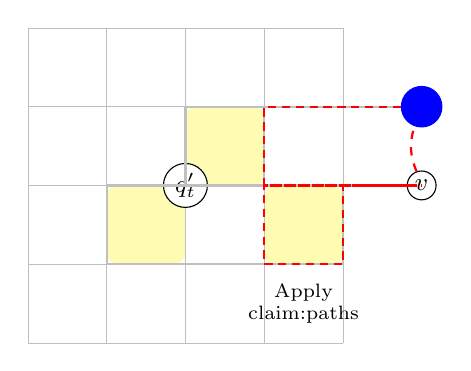
\begin{tikzpicture}[
    vertex/.style = {circle, draw, fill=white, inner sep=1.5pt, font=\small},
    path/.style = {thick, gray!50},
    cycle/.style = {thick, red, densely dashed},
    highlight/.style = {fill=yellow!30, rounded corners}
]
    % Draw the Q_{2r} grid (assuming 2r=4 for visualization)
    \draw[step=1, gray!50, very thin] (0,0) grid (4,4);
    
    % Highlight cells used for paths
    \begin{scope}[on background layer]
        \fill[highlight] (1,1) rectangle (2,2);
        \fill[highlight] (2,2) rectangle (3,3);
        \fill[highlight] (3,1) rectangle (4,2);
    \end{scope}
    
    % Place vertices v and v' outside the grid
    \node[vertex] (v) at (5,2) {$v$};
    \node[vertex, blue] (v') at (5,3) {$v'$};
    \node[vertex] (q) at (2,2) {$q'_t$};
    
    % Draw paths from v and v' to q'_t
    \draw[path] (v) -- (4,2) -- (3,2) -- (2,2);
    \draw[path] (v') -- (4,3) -- (3,3) -- (2,3) -- (2,2);
    
    % Draw auxiliary paths inside Q_{2r} to form the cycle
    \draw[path] (2,2) -- (1,2) -- (1,1) -- (2,1) -- (3,1) -- (4,1) -- (4,2);
    \draw[path] (2,2) -- (2,3) -- (3,3) -- (3,2);
    
    % Draw the odd cycle (length 5: v -> q -> ... -> v)
    \draw[cycle] (v) -- (4,2) -- (3,2) -- (3,1) -- (4,1) -- (4,2) -- (5,2);
    \draw[cycle] (v') -- (4,3) -- (3,3) -- (3,2) -- (4,2) -- (5,2);
    \draw[cycle, dashed] (v) to[bend left=20] (v');
    
    % Annotate the cycle closure using Claim:paths
    \node[align=center, font=\scriptsize] at (3.5, 0.5) {Apply \\ \cref{claim:paths}};
\end{tikzpicture}
\end{document}